\subsection{Muon triggers}
\label{sec:reco-mu-triggers}

Muons are triggered on at L1 using the RPC in the barrel (\modetalt{1.05}) and
the TGC in the endcaps (\modetalt{2.4}). ~\fig{mu-trigger-diag} The chambers are arranged



\begin{figure}[h]
\centering
            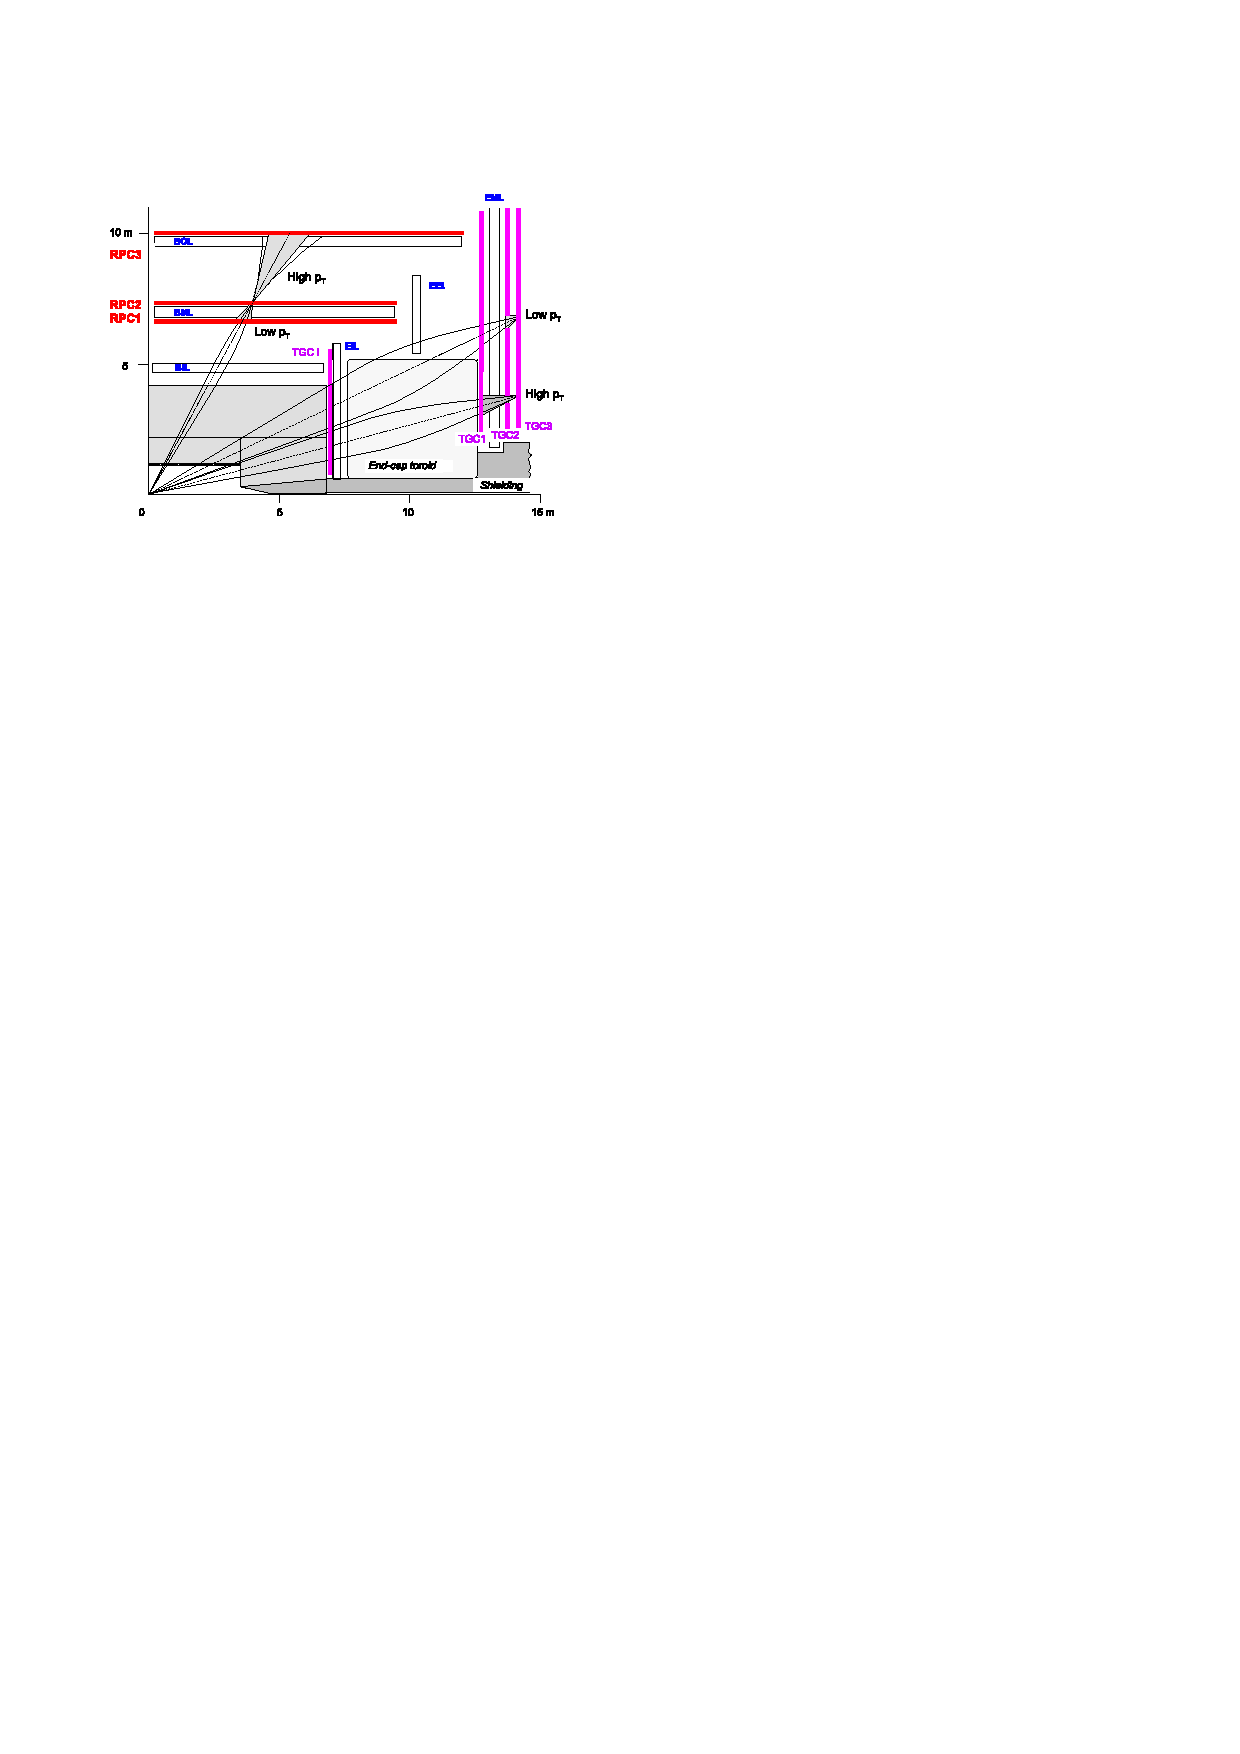
\includegraphics[width=0.8\textwidth]{mu-trigger-diag}
\caption{
Distribution of the Inner Detector material for each sub-detector as a
function of the pseudorapidity. The material of the Pixel and SCT detectors
includes passive material arising from electronics, cabling, cooling and
mechanical support. Figure from~\cite{2012EPJC...72.1849A}.}
\label{fig:mu-trigger-diag}
\end{figure}

- Not affected significantly by pileup, but increased lumi requires tightening of pT selection in 2012.
   - 2011: 18 GeV threshold
   - 2012: 24 GeV, plus isolation: ptcone20/pt<12%. Tracks have to have z0<6mm
   


\subsection{Reconstruction and Identification}
\label{sec:reco-el-reco}
